\section{Bonus : Compléter une grille (3 points)}

Chaque ligne et chaque colonne  de la grille ci-dessous doit contenir les quatre même nombres.

%\begin{multicols}{2}
	\begin{questions}
		\question[1] Recopier la grille et remplacer :
		
		\begin{itemize}
			\item A par le numérateur de $\dfrac{19}{3} - 5$,
			\item B par la somme de $\dfrac{1}{6}$, $\dfrac{1}{3}$ et $\dfrac{1}{2}$,
			\item C par le dénominateur de $\dfrac{19}{6}$,
			\item D par $\dfrac{5}{2} + \dfrac{4}{5} + \dfrac{17}{10}$ ,
		\end{itemize}
	
		\begin{solution}
			\begin{eqnarray*}
				\dfrac{19}{3} - 5 = \dfrac{19}{3} - \dfrac{15}{3} \\
				\dfrac{19}{3} - 5 = \dfrac{4}{3}
 			\end{eqnarray*}
 		
 			\begin{eqnarray*}
 				\dfrac{1}{6} + \dfrac{1}{3} + \dfrac{1}{2} = \dfrac{1}{6} + \dfrac{2}{6} + \dfrac{3}{6}\\
 				\dfrac{1}{6} + \dfrac{1}{3} + \dfrac{1}{2} = \dfrac{6}{6} \\
 				\dfrac{1}{6} + \dfrac{1}{3} + \dfrac{1}{2} = 1 \\
 			\end{eqnarray*}
 		
 		
 			\begin{eqnarray*}
 				\dfrac{5}{2} + \dfrac{4}{5} + \dfrac{17}{10} = \dfrac{25}{10} + \dfrac{8}{10} + \dfrac{17}{10}\\
 				\dfrac{5}{2} + \dfrac{4}{5} + \dfrac{17}{10} = \dfrac{50}{10} \\
 				\dfrac{5}{2} + \dfrac{4}{5} + \dfrac{17}{10} = 5 \\
 			\end{eqnarray*}
 		
 		On a donc $A=4$, $B=1$, $C=6$ et $D=5$
		\end{solution}
	
		\question[2] Compléter la grille (Plusieurs réponses sont possibles).
		\begin{solution}
			\begin{center}
				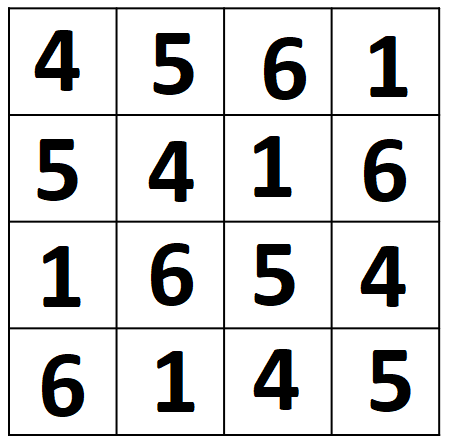
\includegraphics[scale=0.5]{img/grille2}
			\end{center}
		\end{solution}
		
	\end{questions}

	\begin{center}
		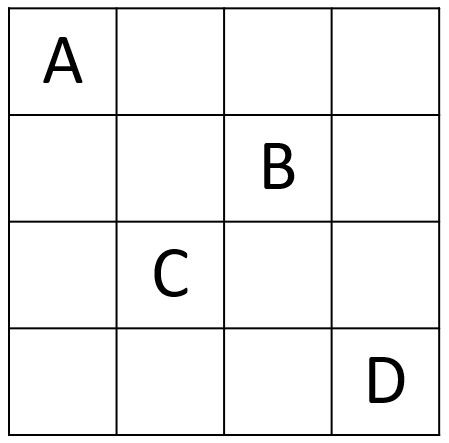
\includegraphics[scale=0.5]{img/grille}
	\end{center}
%\end{multicols}